% -*- root: ../main.tex -*-

%  piano di lavoro adottato. A tal fine, per ogni attività svolta durante la preparazione dell'elaborato (ad esempio: studio di una tecnologia, progettazione di un componente, implementazione di un algoritmo ecc. . . ) deve essere chiarita la collocazione temporale e devono essere indicate le risorse impiegate per svolgerla (giorni/uomo). I candidati possono ricorrere a opportuni diagrammi come quello di Gantt.

\chapter{Piano di lavoro}
Il lavoro è stato svolto utilizzando un approccio Scrum, con quattro sprint, più uno iniziale incentrato sullo studio delle tecnologie.
\begin{figure}[H]
    \caption{Gantt Chart}
    \label{fig:Gantt}
    \centering
    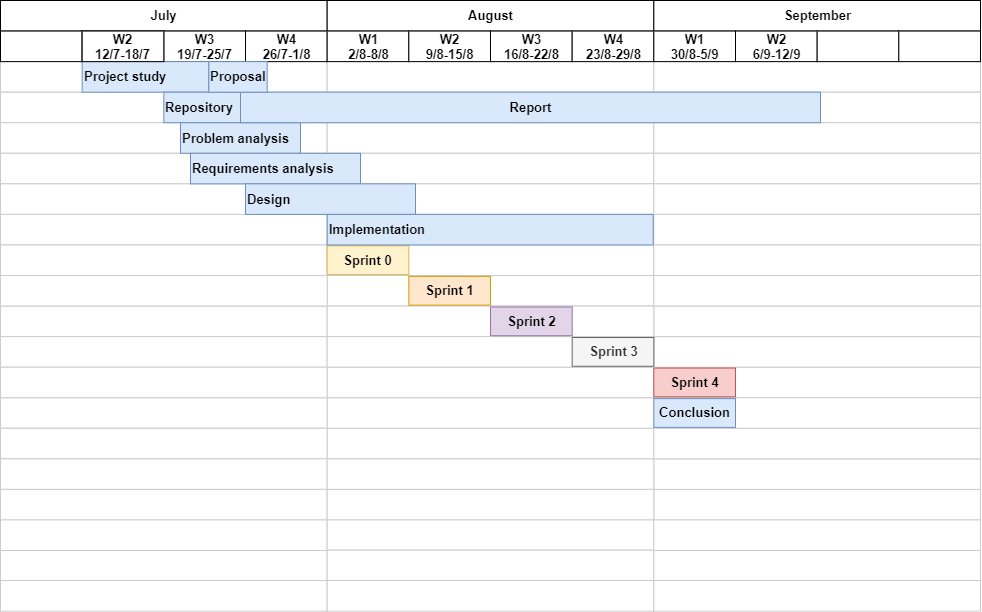
\includegraphics[width=1\textwidth]{DrawIo/GanttChart.png}
\end{figure}